\documentclass[en]{../../../eplsummary}

\usepackage{siunitx}
\usepackage{circuitikz}

\newcommand*\mean[1]{\overline{#1}}
\newcommand*\equal{=} % hack to have = in tikz

\hypertitle{Analog Electronics}{8}{ELEC}{2532}
{Antoine Paris}
{Denis Flandre}

\section{Electronic noise}
The reference for this section is~\cite[chapter~11]{gray}.
This section assumes the reader is familiar with concepts of variance,
covariance, stationarity, power spectral density, Wiener-Kintchine
theorem, etc. Please refer to the stochastic processes course otherwise.

\subsection{Sources of noise}
The notation $\mean{x^2}$ corresponds to a mean-square variation around
the average value $\mu_x$
\begin{align*}
    \mean{x^2}  &= \mean{(x-\mu_x)^2} \\
                &= \lim_{T\to\infty}\frac{1}{T}\int_0^T (x-\mu_x)^2
                \mathrm{d}t.
\end{align*}
In other words, $\mean{x^2}$ is the variance of $x$, $\sigma^2_x$.

\subsubsection{Thermal noise}
In conventional resistors, it is due to the \emph{random thermal motion of
the electrons} and is unnafected by the presence or absence of direct
current. In a resistor $R$, thermal noise can be represented by a series
voltage generator $\mean{v^2}$ or by a shunt current generator $\mean{i^2}$.
\begin{align*}
    \mean{v^2} &= 4kTR\Delta f \\
    \mean{i^2} &= 4kT\frac{1}{R}\Delta f,
\end{align*}
where $k$ is the Boltzmann's constant, $T$ the absolute temperature (i.e. in
Kelvin) and $\Delta f$ the bandwidth in Hertz.
From this, it is clear that thermal noise is a \textbf{white noise}. Indeed,
its power spectral density is given either by $4kTR$ in \SI{}{\volt\squared
\per\hertz} or by $4kT\frac{1}{R}$ in \SI{}{\ampere\squared\per\hertz} and
is constant as a function of frequency\footnote{As a reminder, the power
spectral density is defined as the Fourier transform of the auto-covariance
function of a weak-sense stationary random process. A constant power spectral
density thus means that the auto-covariance function is a delta, i.e. that
the given random process at different time instants is uncorrelated.}
(this is true up to \SI{1e13}{\hertz}).
In a resistor $R$, thermal noise can be represented as in figure
~\ref{fig:thermal-noise-repr}.
%FIXME: I am not quite sure to understand this model, what current delivers?
%I suppose it's the rms and not the ms as seems to be indicated in the figure
%below
\begin{figure}[ht]
    \centering
    \begin{circuitikz}
        \draw
        (0,0) to[short, o-] (0,-0.5)
        (0,-0.5) to[R, l=$R$] (0,-2)
        (0,-3.5) to[V, v=$\mean{v^2}$] (0,-2)
        (0,-3.5) to[short, -o] (0,-4)
        
        (5,0) to[short, o-*] (5,-0.5)
        (5,-0.5) to[R, l=$R$] (5,-3.5)
        (5,-3.5) to[short, *-o] (5,-4)
        (5,-0.5) -- (7,-0.5) to[I, i=$\mean{i^2}$] (7,-3.5) -- (5,-3.5)
        ;
    \end{circuitikz}
    \caption{Representations of thermal noise.}
    \label{fig:thermal-noise-repr}
\end{figure}
Finally, the the amplitude distribution of thermal noise is
\textbf{Gaussian}.

\paragraph{Superposition}
When two sources of voltage noises are in series, they can be grouped
in a equivalent source of voltage noise $\mean{v^2_e}$ as illustrated below.

\begin{center}
    \begin{circuitikz}
        \draw
        (0,0) to[short, o-] (0,-0.5)
        (0,-2) to[V, v=$\mean{v_1^2}$] (0,-0.5)
        (0,-3.5) to[V, v=$\mean{v_2^2}$] (0,-2)
        (0,-3.5) to[short, -o] (0,-4)
        
        (2,-2.5) node[label=$\to$]{}
        
        (4,0) to[short, o-] (4,-0.5)
        (4,-3.5) to[V, v=$\mean{v_e^2}$] (4,-0.5)
        (4,-3.5) to[short, -o] (4,-4)
        ;
    \end{circuitikz}
\end{center}
The relation between $\mean{v^2_e}$ and $\mean{v_1^2}$ and $\mean{v_2^2}$
depends on the relation between $v_1$ and $v_2$.

\begin{itemize}
    \item Non-correlated sources:
    \[ \mean{v^2_e} = \mean{v^2_1} + \mean{v^2_1} \]

    \item Fully correlated sources:
    \[ \mean{v^2_e} = \mean{(v_1+v_2)^2} \]

    \item Partially correlated sources:
    let $v_2 = v_{22} + v_{21}$ where $v_{22}$ is non-correlated with $v_1$
    and $v_{21}$ is fully correlated with $v_1$. In this case,
    \[ \mean{v^2_e} = \mean{(v_1 + v_{21})^2} + \mean{v^2_{22}}. \]
\end{itemize}

\subsubsection{Shot noise}
Shot noise is always associated with a direct-current flow and is present in
diodes, MOS transistors and bipolar transistors (i.e. devices for which
a potential barrier across a junction exists). The passage of each carrier
across the junction can be modeled as a random event (which depends on
carrier's energy, direction, etc). The external current is thus composed of
a large number of random independent current pulses. Noting $I_J$ the average
current across the junction, the noise current has a mean square given by
\[ \mean{i^2} = 2qI_J\Delta f \]
where $q$ is the electronic charge. As for thermal noise, this is a
\textbf{white noise} with a \textbf{Gaussian} amplitude distribution.
A small-signal model of a diode including the effect of shot noise is
illustrated in figure~\ref{fig:shot-noise-diode-repr}.
\begin{figure}[ht]
    \centering
    \begin{circuitikz}
        \draw
        (2,0) to[short, o-] (2,-0.5)
        (2,-0.5) to[D, i=$I_D$] (2,-2.5)
        (2,-2.5) to[short, -o] (2,-3)
        
        (5,0) -- (8,0) to[I, i=$\mean{i^2}\equal2qI_D\Delta f$] (8,-3)
        (8,-3) -- (5,-3) to[R, l=$r_d\equal\frac{kT}{qI_D}$] (5,0)
        ;
    \end{circuitikz}
    \caption{Diode small signal model including the effect of shot noise.
    Note that the small signal resistance $r_d$ of the diode is not an actual
    resistance (i.e. that's just a model of the diode). As such, it is not
    a source of thermal noise.}
    \label{fig:shot-noise-diode-repr}
\end{figure}
%TODO: why polarity of the source doesn't matter (related to above fixme)
Finally, shot noise is non-correlated with thermal noise. Because shot noise
and thermal noise are both Gaussian, this means that they are independent.

\subsubsection{Flicker noise}
Flicker noise (also called pink noise, or $1/f$ noise) is a type of noise
found in all active devices, as well as in some discrete passive elements
such as carbon resistors. The origins of flicker noise are varied, but it is
caused mainly by traps associated with contamination and crystal defects.
Flicker noise is always associated with a flow of direct current, the noise
current has a mean square given by
\[ \mean{i^2} = K_1\frac{I^a}{f^a}\Delta f \]
where $\Delta f$ is a small\footnote{Indeed, $\mean{i^2} = \sigma^2_i$ is
rigorously defined as the integral of the power spectral density on the
bandwidth of interest. Because the power spectral density here is not flat,
the formula is only an approximation for small $\Delta f$.} bandwidth around
$f$, $I$ is the direct current, $K_1$, $a$ and $b$ are technology parameters.
At the opposite of thermal noise and shot noise, flicker noise is \textbf{not
white} (hence the name pink) and often has a \textbf{non-Gaussian} amplitude
distribution.

%TODO: might be better in a table in fact...
\subsubsection{Summary}
A summary of the different noise sources is given in
figure~\ref{fig:noise-summary}.

\begin{figure}[ht]
    \centering
    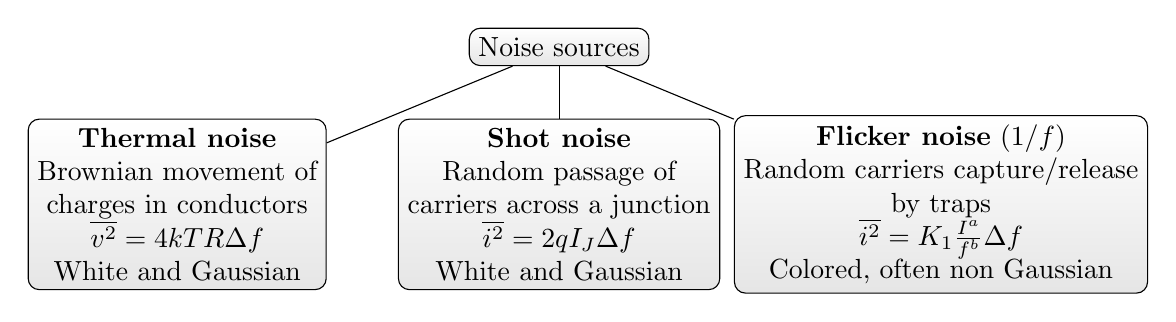
\begin{tikzpicture}[level distance=2cm,
        level 1/.style = {sibling distance = 0.4\textwidth},
        every node/.style = {shape=rectangle, rounded corners,
        draw, align=center,
        top color=white, bottom color=gray!20}]

        \node {Noise sources}
            child { node {\textbf{Thermal noise}\\
            Brownian movement of\\
            charges in conductors\\
            $\mean{v^2} = 4kTR\Delta f$\\
            White and Gaussian}  }
            child { node {\textbf{Shot noise}\\
            Random passage of\\
            carriers across a junction\\
            $\mean{i^2} = 2qI_J\Delta f$\\
            White and Gaussian} }
            child { node {\textbf{Flicker noise} ($1/f$)\\
            Random carriers capture/release\\
            by traps\\
            $\mean{i^2} = K_1\frac{I^a}{f^b}\Delta f$\\
            Colored, often non Gaussian} };    
    \end{tikzpicture}
    \caption{Summary of the different noise sources.}
    \label{fig:noise-summary}
\end{figure}

\subsection{Noise models of Integrated-Circuit Components}
\subsubsection{Resistors}
Monolithic and thin-film resistors display thermal noise. This is illustrated
in figure~\ref{fig:thermal-noise-repr}.

\subsubsection{Capacitors and inductors}
There are \emph{no sources of noise} in \emph{ideal} capacitors or
inductors. In practice, however, real components have parasitic resistances
that does display thermal noise.

\subsubsection{Junction Diode}
A small-signal model of the diode that includes the effect of shot noise was
already given in figure~\ref{fig:shot-noise-diode-repr}. This one, however,
does not take into account neither the series parasitic resistance of the
diode (which will display thermal noise) or flicker noise. A more complete
model is given in figure~\ref{fig:diode-noise-model}.

\begin{figure}[ht]
    \centering
    \begin{circuitikz}
        \draw 
        (1.5, 3.3) to[short, o-] (1.5, 3) 
        (1.5, 3) to[V, v=$\mean{v^2_s}\equal4kTr_s\Delta f$] (1.5, 1.5)
        (1.5, 1.5) to[R, l=$r_s$] (1.5, 0) to[short, -*] (1.5, 0)
        (0,0) -- (3,0) to[I, i=$\mean{i^2}\equal2qI_D\Delta f
        + K\frac{I_D^a}{f^b}\Delta f$] (3,-3)
        (3,-3) -- (0,-3) to[R, l=$r_d\equal\frac{kT}{qI_D}$] (0,0)
        (1.5, -3) to[short, -o] (1.5, -3.3)
        ;
    \end{circuitikz}
    \caption{Complete diode small-signal model equivalent circuit with noise
    sources.}
    \label{fig:diode-noise-model}
\end{figure}

\subsubsection{Bipolar transistor}
A small-signal model equivalent circuit with noise sources for a bipolar transistor
is given in figure~\ref{fig:bjt-noise-model}. This model contains the following
noise sources:
\begin{itemize}
	\item $\mean{v^2_b}$: thermal noise associated with the
	parasitic resistance of the base connection
	\[ \mean{v^2_b} = 4kTr_b\Delta f. \]
	\item $\mean{i^2_c}$: random transit time through the base (i.e. shot noise)
	\[ \mean{i^2_c} = 2qI_C\Delta f. \]
	\item $\mean{i^2_b}$: random carrier injection in emitter (i.e shot noise).
	Experimentally, it can also be seen that the base current is sensitive to
	flicker noise and telegraph noise (neglected in this course)
	\[ \mean{i^2_b} = 2qI_b\Delta f + K_1\frac{I_b^a}{f^b}\Delta f. \]
\end{itemize}

\begin{figure}[ht]
    \centering
    \begin{circuitikz}
        \draw
        (0, 2) to[short, o-, l=$B$] (0, 2) to[R, l=$r_b$] (2, 2)
        (2, 2) to[V, v=$\mean{v_b^2}$] (4, 2)
        (0, 0) to[short, o-] (0, 0) -- (4, 0)
        (4, 0) to[I, i=$\mean{i_b^2}$] (4, 2)
        (4, 2) -- (5.5, 2) to[R, l_=$r_\pi$] (5.5, 0) -- (4, 0)
        (5.5, 2) -- (7, 2) to[C, l_=$C_\pi$, v^=$v_\pi$] (7, 0) -- (5.5, 0)
        (7, 0) to[short, -, l=$E$] (9, 0)
        (9, 2) to[I, i=$g_mv_\pi$] (9, 0)
        (9, 2) -- (11, 2) to[R, l=$r_o$] (11, 0) -- (9, 0)
        (11, 0) -- (13, 0) to[I, i=$\mean{i_c^2}$] (13, 2) -- (11, 2)
        (13, 0) to[short, -o] (13.5, 0)
        (13, 2) to[short, -o, l=$C$] (13.5, 2)
        ;
    \end{circuitikz}
    \caption{Bipolar transistor small-signal equivalent circuit
    with noise sources.}
    \label{fig:bjt-noise-model}
\end{figure}

The power spectral density associated with the noise source $\mean{i_b^2}$ (i.e
$\mean{i_b^2}/\Delta f$) is illustrated in figure~\ref{fig:corner-frequency}.
\begin{figure}
	\centering
	\includegraphics[width=0.6\textwidth]{figures/corner-frequency.png}
	\caption{Power spectral density of the base-current noise generator in a
	bipolar transistor. At low frequency, $1/f$ noise dominates while at higher
	frequency, shot noise dominates. $f_a$ is called the flicker noise
	\emph{corner} frequency.}
	\label{fig:corner-frequency}
\end{figure}

\section{Active filters}

\section{Voltage references}

\section{DAC}

\section{ADC}

\nocite{*}
\bibliographystyle{plain}
\bibliography{biblio}

\end{document}
